\section{Data selection}
The  radio baseline  we  observe is  a  results of  several known  and
unknown effects. A daily modulation is due to the temperature and will
be  corrected  for in  section~\ref{sec:tempdep}.   Humidity seems  to
affect  a   lot  the  baseline,  but  the   parameterization  is  more
difficult. We also  notice some large change of  the baseline that can
be due  to storm.  We  present in this  section the cut we  operate to
clean the data and keep the  period when the baseline is only affected
by  the temperature.\\In  principle  we could  make  cuts on  humidity
value, but the  monitoring information is not always  present. We then
make cuts on the shape of  the radio baseline and select the days when
the variations are smooth. The figure~\ref{fig:selected} shows the day
selected for each station. The date are also reported in the appendix.

\begin{figure}[!ht]
  \centering
  \hspace*{-3ex}
  \subfigure{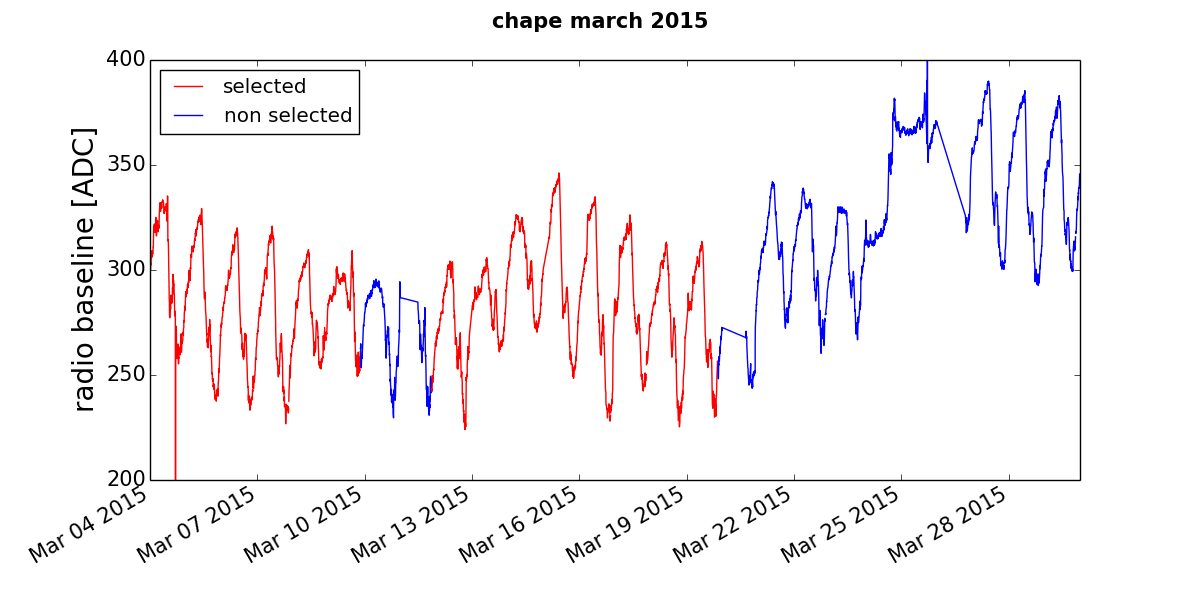
\includegraphics[width=0.49\linewidth]{chapemarch2015.png}}
  \subfigure{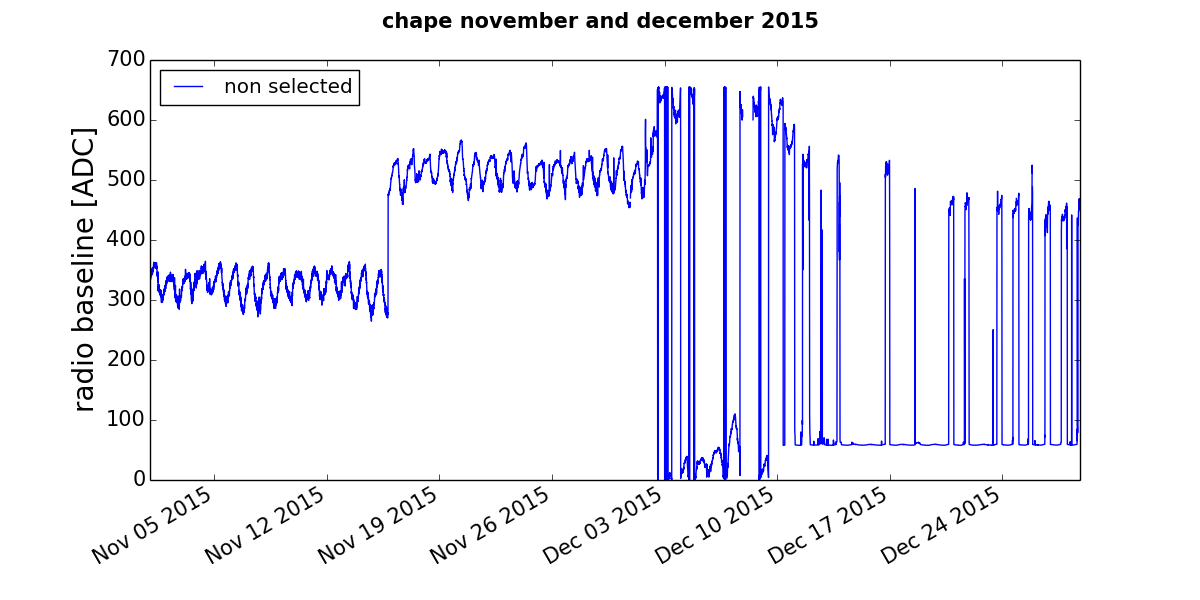
\includegraphics[width=0.49\linewidth]{chapenovdec2015.png}}\\
  \subfigure{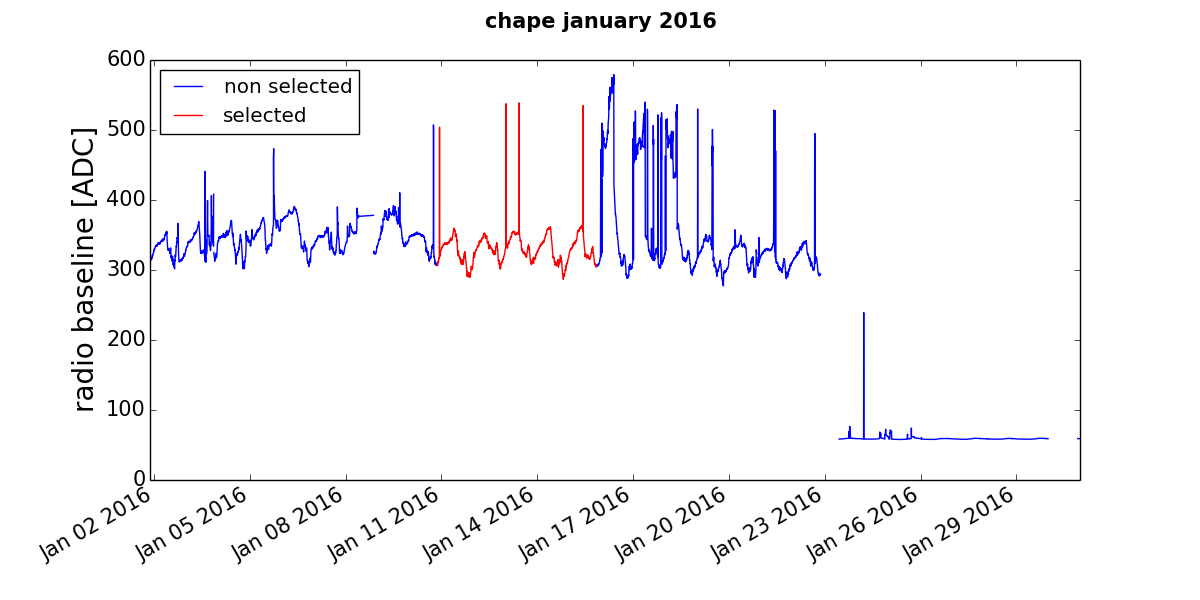
\includegraphics[width=0.49\linewidth]{chapejan2016.png}}
  \subfigure{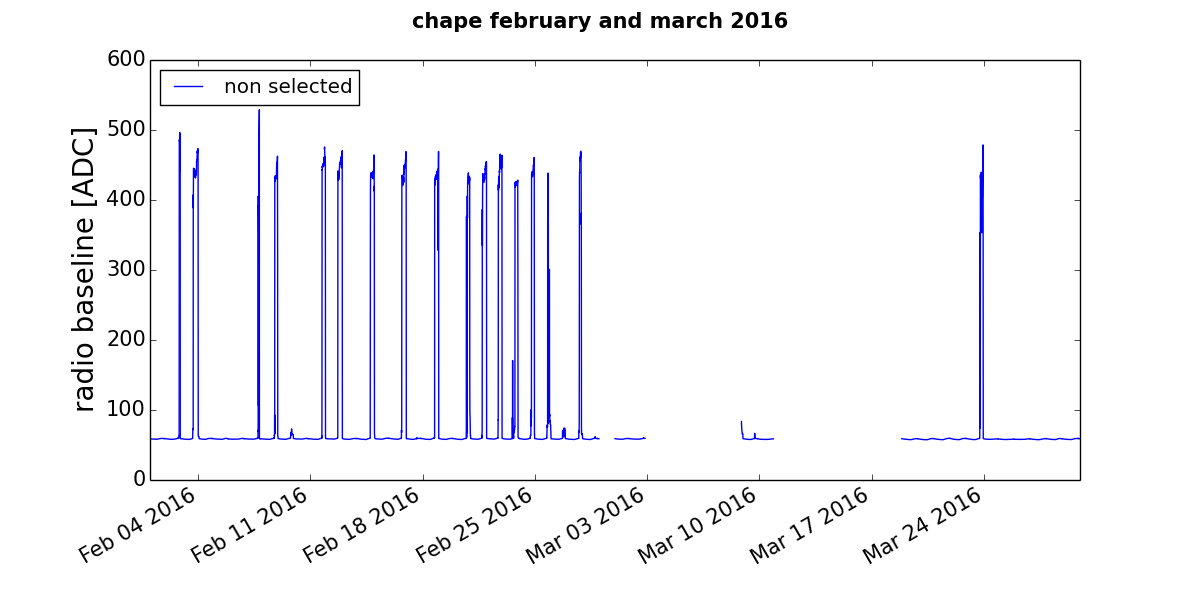
\includegraphics[width=0.49\linewidth]{chapefebmarch2016.png}}
  \caption{Selected period in red for Popey}
  \label{fig:selectedchape}
\end{figure}

\begin{figure}[!ht]
  \centering
  \hspace*{-3ex}
  \subfigure{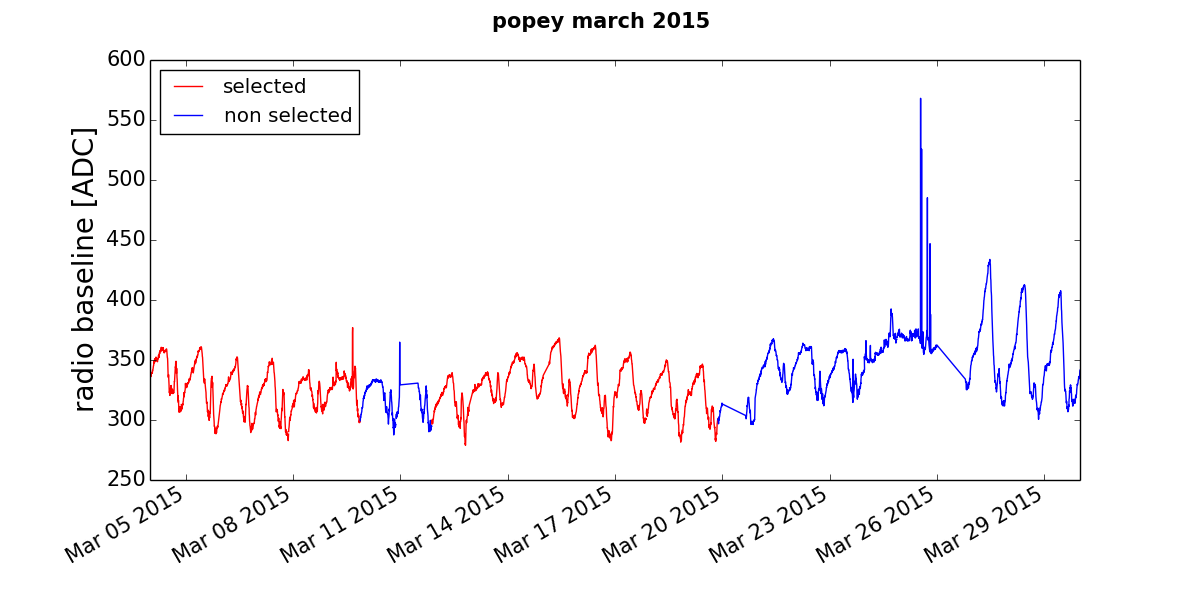
\includegraphics[width=0.49\linewidth]{popeymarch2015.png}}
  \subfigure{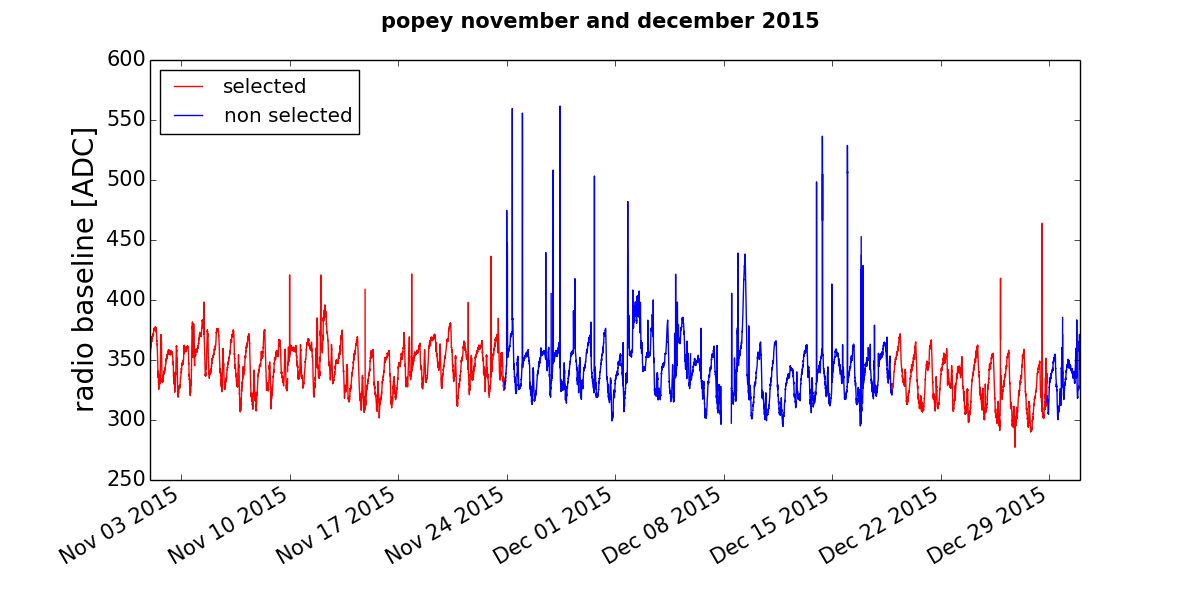
\includegraphics[width=0.49\linewidth]{popeynovdec2015.png}}\\
  \subfigure{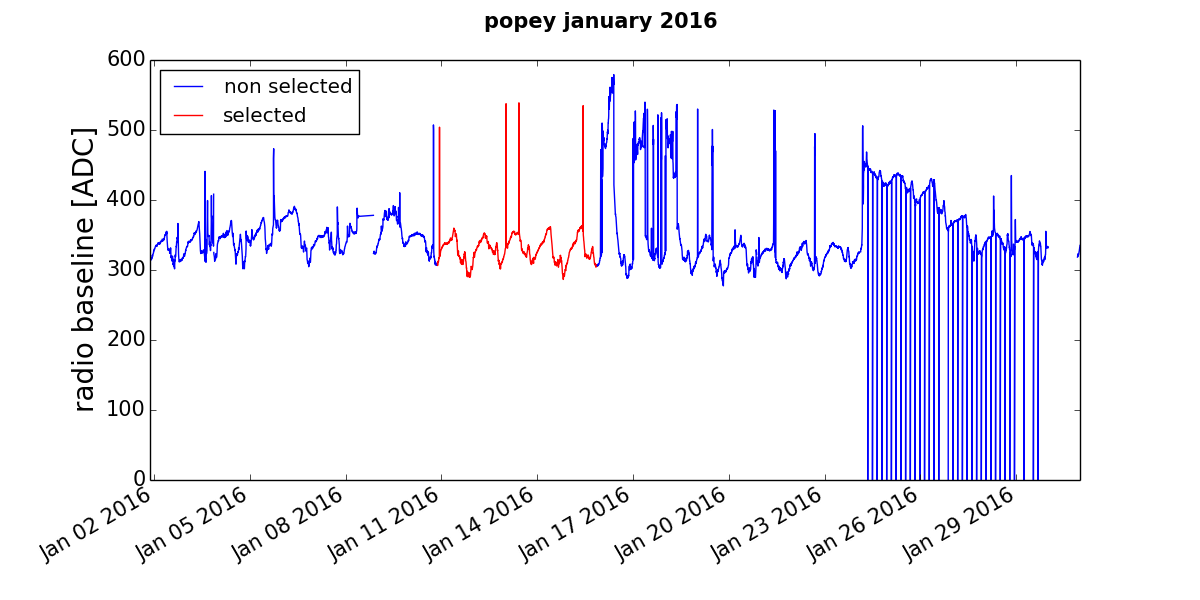
\includegraphics[width=0.49\linewidth]{popeyjan2016.png}}
  \subfigure{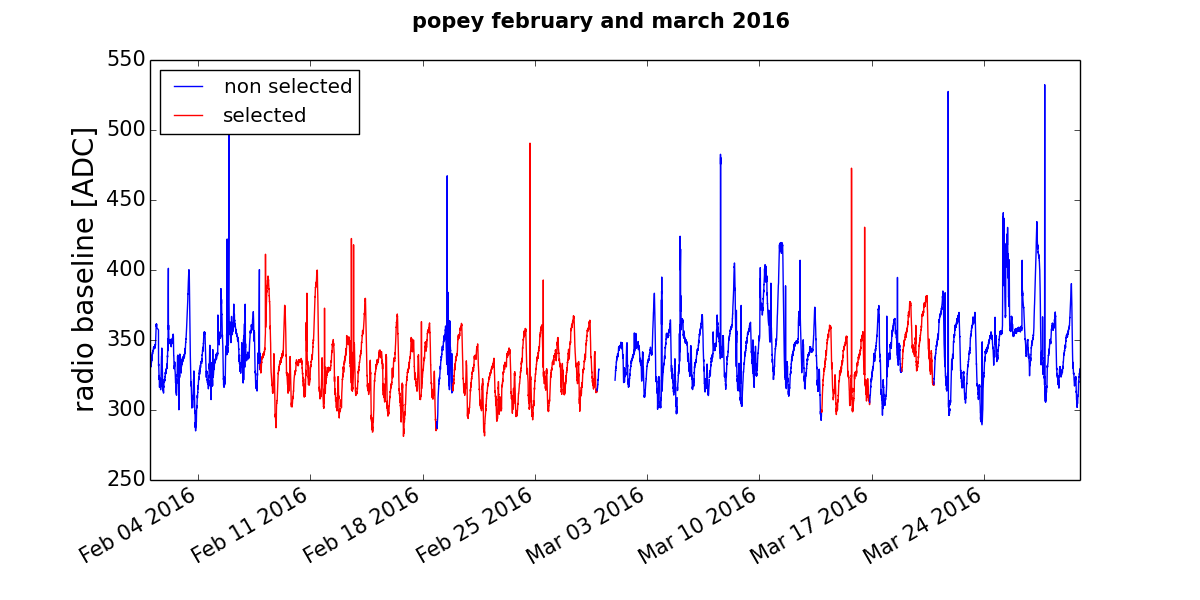
\includegraphics[width=0.49\linewidth]{popeyfebmarch2016.png}} 
  \caption{Selected period in red for Popey}
 \label{fig:selectedpopey}
\end{figure}
At the end we selected 


